% Options for packages loaded elsewhere
\PassOptionsToPackage{unicode}{hyperref}
\PassOptionsToPackage{hyphens}{url}
%
\documentclass[
]{article}
\usepackage{amsmath,amssymb}
\usepackage{lmodern}
\usepackage{iftex}
\ifPDFTeX
  \usepackage[T1]{fontenc}
  \usepackage[utf8]{inputenc}
  \usepackage{textcomp} % provide euro and other symbols
\else % if luatex or xetex
  \usepackage{unicode-math}
  \defaultfontfeatures{Scale=MatchLowercase}
  \defaultfontfeatures[\rmfamily]{Ligatures=TeX,Scale=1}
\fi
% Use upquote if available, for straight quotes in verbatim environments
\IfFileExists{upquote.sty}{\usepackage{upquote}}{}
\IfFileExists{microtype.sty}{% use microtype if available
  \usepackage[]{microtype}
  \UseMicrotypeSet[protrusion]{basicmath} % disable protrusion for tt fonts
}{}
\makeatletter
\@ifundefined{KOMAClassName}{% if non-KOMA class
  \IfFileExists{parskip.sty}{%
    \usepackage{parskip}
  }{% else
    \setlength{\parindent}{0pt}
    \setlength{\parskip}{6pt plus 2pt minus 1pt}}
}{% if KOMA class
  \KOMAoptions{parskip=half}}
\makeatother
\usepackage{xcolor}
\IfFileExists{xurl.sty}{\usepackage{xurl}}{} % add URL line breaks if available
\IfFileExists{bookmark.sty}{\usepackage{bookmark}}{\usepackage{hyperref}}
\hypersetup{
  pdftitle={How has the Brazilian Amazon been constructed as a problem? An analysis of presidential speeches since 1985},
  pdfauthor={Livio Silva-Muller; Henrique Sposito},
  hidelinks,
  pdfcreator={LaTeX via pandoc}}
\urlstyle{same} % disable monospaced font for URLs
\usepackage[margin=1in]{geometry}
\usepackage{graphicx}
\makeatletter
\def\maxwidth{\ifdim\Gin@nat@width>\linewidth\linewidth\else\Gin@nat@width\fi}
\def\maxheight{\ifdim\Gin@nat@height>\textheight\textheight\else\Gin@nat@height\fi}
\makeatother
% Scale images if necessary, so that they will not overflow the page
% margins by default, and it is still possible to overwrite the defaults
% using explicit options in \includegraphics[width, height, ...]{}
\setkeys{Gin}{width=\maxwidth,height=\maxheight,keepaspectratio}
% Set default figure placement to htbp
\makeatletter
\def\fps@figure{htbp}
\makeatother
\setlength{\emergencystretch}{3em} % prevent overfull lines
\providecommand{\tightlist}{%
  \setlength{\itemsep}{0pt}\setlength{\parskip}{0pt}}
\setcounter{secnumdepth}{-\maxdimen} % remove section numbering
\newlength{\cslhangindent}
\setlength{\cslhangindent}{1.5em}
\newlength{\csllabelwidth}
\setlength{\csllabelwidth}{3em}
\newlength{\cslentryspacingunit} % times entry-spacing
\setlength{\cslentryspacingunit}{\parskip}
\newenvironment{CSLReferences}[2] % #1 hanging-ident, #2 entry spacing
 {% don't indent paragraphs
  \setlength{\parindent}{0pt}
  % turn on hanging indent if param 1 is 1
  \ifodd #1
  \let\oldpar\par
  \def\par{\hangindent=\cslhangindent\oldpar}
  \fi
  % set entry spacing
  \setlength{\parskip}{#2\cslentryspacingunit}
 }%
 {}
\usepackage{calc}
\newcommand{\CSLBlock}[1]{#1\hfill\break}
\newcommand{\CSLLeftMargin}[1]{\parbox[t]{\csllabelwidth}{#1}}
\newcommand{\CSLRightInline}[1]{\parbox[t]{\linewidth - \csllabelwidth}{#1}\break}
\newcommand{\CSLIndent}[1]{\hspace{\cslhangindent}#1}
\usepackage{booktabs}
\usepackage{longtable}
\usepackage{array}
\usepackage{multirow}
\usepackage{wrapfig}
\usepackage{float}
\usepackage{colortbl}
\usepackage{pdflscape}
\usepackage{tabu}
\usepackage{threeparttable}
\usepackage{threeparttablex}
\usepackage[normalem]{ulem}
\usepackage{makecell}
\usepackage{xcolor}
\ifLuaTeX
  \usepackage{selnolig}  % disable illegal ligatures
\fi

\title{How has the Brazilian Amazon been constructed as a problem? An
analysis of presidential speeches since 1985}
\author{Livio Silva-Muller\footnote{Phd Candidate, The Graduate
  Institute Geneva,
  \href{mailto:livio.silva@graduateinstitute.ch}{\nolinkurl{livio.silva@graduateinstitute.ch}}} \and Henrique
Sposito\footnote{Phd Candidate, The Graduate Institute Geneva,
  \href{mailto:henrique.sposito@graduateinstitute.ch}{\nolinkurl{henrique.sposito@graduateinstitute.ch}}}}
\date{April 2022}

\begin{document}
\maketitle
\begin{abstract}
This paper \ldots{}
\end{abstract}

\pagebreak

\hypertarget{introduction}{%
\section{1 Introduction}\label{introduction}}

The Amazon needs to be protected from foreign interests. The Amazon
needs to be exploited for its natural resources. The Amazon should be
preserved as a standing ecosystem. Historically, different Brazilian
federal government proposed diverse policies to deal with the Amazon.
Each of these policies contain an implicit assumption of what needs to
be solved, or in other words, it represents the region, the forest, or
the peoples as a particular problem. In the three examples above, the
Amazon is represented as an issue of national sovereignty, economic
integration, and environmental conservation, respectively. Each of these
constructions, and their proposed solutions, have been described as
policy cycles of Brazilian governments (Acker 2014; Hecht and Cockburn
1990; Hochstetler and Keck 2007). However, policy cycles are usually
represented monolithically, advancing a view that specific governments
see the Amazon as an instance of only one specific problem. Albeit the
current academic calls to understand the environment as a
social-cultural construction and to identify the effect of culture for
environmental outcomes (Polain de Waroux et al. 2021), we lack empirical
accounts of how the Brazilian Amazon has been constructed as a problem
over time and across locations, and how this varies.

In this article, we investigate how the Brazilian Amazon has been
constructed as a problem in political discourses. Building on Hirschman
(1963) concept of chosen problems in policy making, we propose a
framework to identify how problem-construction varies over time, by
location, and between and within governments. Although
problem-construction takes place in a series of instances (e.g.~policy
committees, legislative bodies, media, etc.), we analyze the case of
political discourse by Brazilian presidents since 1985. We opt for
presidential speeches for three reasons. First, political discourses at
the top have the power to introduce and justify public policy, as well
as shape its perception to broad audiences (Zarefsky 2004). In turn,
policy perception is key for policy adoption and implementation (Alesina
and Giuliano 2009). The literature has shown that deforestation rates in
Brazil are more responsive to the government's environmental policy than
exogenous factors as market fluctuations (Assunção, Gandour, and Rocha
2015; Capobianco 2019, 2021). Thus, understanding how policy comes about
discursively is important. Second, environmental discourse at the top
can help expand or restrict what types of behaviors are accepted in the
ground. When Brazilian presidents speak about the Amazon it not only
makes headlines, nationally and internationally, but also incites
responses, shapes expectations, and feeds into the behavior of many
actors involved with the Amazon, from investors to agribusiness to local
farmer(Brice and Smith 2021; Harris 2021; Miranda 2021). This is
especially pertinent for deforestation as previous research found that
policy expectations, generated from material and discursive governmental
practices, are a crucial factor in decisions to deforest at the ground
(Capobianco 2019; Campbell 2015). Unpacking discourse at the top might
help us raise hypotheses about environmental outcomes that are
culturally situated. Finally, as our theoretical framework suggests,
problem-construction varies by geographic location. Presidential
discourses take place in a series of sites with diverse audiences: from
launching a new bridge in a small municipality in the middle of the
Amazon, to a keynote speech in a business association in São Paulo, to
the UN general assembly in New York city. Working with presidential
discourses allows us to identify this variation in meaningful ways and
better how the Amazon is socially constructed.

To investigate how the Brazilian Amazon has been constructed as a
problem in political discourses, we create a dataset containing 6130
official presidential speeches by all Brazilian presidents since 1985.
We subset the dataset by identifying Amazonian related statements within
these speeches. We find that 2014 sections in these discourses refer to
the Amazon at least once. We then develop a codebook grounded on
Amazonian historiography to code how each of these statements constructs
the Amazon as a particular problem. We use this codebook to manually
code a randomly selected training set of the Amazonian related
statements. Using R, we then train a supervised machine-learning model
in the hand-coded set and automatically label the remaining set of
Amazonian statements. We then conduct a descriptive and inferential
analysis of this data, tying our findings to endogenous and exogenous
events related to deforestation.

(Summarize findings, conceptual contribution, and empirical
contribution). Conceptually, our approach is underpinned by a
constructivist view of policy making, which allocates agency to
different actors in building policy discursively. Empirically, we
provide the first comprehensive overview of how the Brazilian Amazon has
been constructed as a problem in presidential speeches.

This article proceeds as follows: first, we review Amazonian literature
to identify the main ways in which it was constructed as a problem. We
then propose a theoretical framework to understand problem-construction.
In the methodology section, we operationalize our framework and the
Amazonian problem-constructions. Section four portrays our main results
over time and by speaker. Finally, we conclude by discussing our
findings and proposing future research.

\hypertarget{amazonian-policy-cycles-discourse-and-problem-construction}{%
\section{2 Amazonian policy-cycles, discourse, and
problem-construction}\label{amazonian-policy-cycles-discourse-and-problem-construction}}

\hypertarget{literature-review-policy-cycles-in-the-amazonian-literature}{%
\subsection{2.1 Literature Review: policy-cycles in the Amazonian
literature}\label{literature-review-policy-cycles-in-the-amazonian-literature}}

For the purposes of this article, we understand Amazonian literature as
the body of research by social and environmental scientists that tells
the story of diverse policies adopted to solve problems in the region.
The three main policy-cycles we identify in Amazonian literature are:
national sovereignty, economic integration, and environmental
conservation. We tie each one of them to a specific problem and
consequently a solution. We close the sub-section reviewing the
relationship between policy, presidential discourse, and environmental
problems.

\hypertarget{national-sovereignty}{%
\subsubsection{2.1.1 National sovereignty}\label{national-sovereignty}}

In The Fate of the Forest: Developers, Destroyers, and Defenders of the
Amazon, Hecht and Cockburn write that all over the world tropical
forests are destroyed, but ``what imbues the case of the Amazon with
such passion is the symbolic content of the dreams it ignites'' (1990,
1). It started with the first natural history of the New World, by
Oviedo in 1535, who recounts the stories of conquest of local
populations and gold hoarders. The dream of fortunes to be found in the
Eldorado composed the imaginaries of \emph{bandeirantes}\footnote{B\emph{andeirantes}
  means ``flag-carriers'', the word is used to designate Portuguese
  colonials and later Brazilian explorers, expanding the Brazilian
  territory beyond what the Tordesillas Treaty established. The treaty
  allocated almost the whole Amazonian territory to the Spanish Empire,
  the bandeirantes took much of the territory afterwards.} from the
southeast of Brazil and colonizers from everywhere else. It rendered the
territory the venue for aspiration and object of an intense scramble in
the subsequent centuries, defined as ``a (\ldots) form of nation
building (\ldots)'' (Hecht and Cockburn 1990, preface). The Portuguese
empire and subsequently the Brazilian monarchy were concerned with
establishing their territory. In the process of securing Amazonian
borders, Brazil thwarted ``the imperial ambitions of France, Britain,
the United States, Belgium, Bolivia, and Peru'' (Hecht 2013, 8), and
when the dust settled and the scramble was over, half of the Amazon
emerged Brazilian. While Brazilian military diplomacy was very
successful, the process did not come without its traumas. A significant
experience were the negotiations with Bolivia in 1902 to secure the
Amazonian state of Acre, during which they found out about American
attempts to trick Brazil(Hecht and Cockburn 1990). This case was still
part of the memory of the generals who led the country during the
military dictatorship of 1964 and wanted to protect Brazil's sovereignty
over the Amazon from the communist threat during the Cold War(Garfield
2013). As we move from a world where non-state actors gain importance in
environmental governance and international politics generally
(Silva-Muller and Faul 2022; Andonova 2014; Westerwinter 2021), the
sovereignty problem becomes more varied. Multiple non-state actors
(NGOs, foundations, IOs, and so on) join the conversation about
Amazonian policies more substantially as the military dictatorship
starts to end (Hochstetler 2021; Capobianco 2019; Franchini and Viola
2019). Threads to national sovereignty, consequently, can be interpreted
as coming from a different set of actors than before. False claims about
Brazilian policies in international and domestic fora, for instance, are
often tied to strategies of `internationalizing' the Amazon. Relatedly,
mentions of Amazonian myths which have been debunked as the `Earth of
the Lungs', are also tied to internationalizing strategies.

The sovereignty problem advances the view that the Brazilian Amazon is
Brazilian and foreign presence, non-state presence and alleged lies are
part of a broader strategy to internationalize the region. The policy
solutions relate to close monitoring of the borders, strict regimes
related to entry in the region, and combating alleged disinformation
about the Amazon nationally and internationally.

\hypertarget{economic-integration}{%
\subsubsection{2.1.2 Economic integration}\label{economic-integration}}

The dictatorships of Vargas (1937-46) and the military (1964-89) took
over the task of modernizing the Amazon. In 1966, the Brazilian Military
dictatorship launched Operation Amazon, a policy to modernize the region
based on a set of assumptions (Acker 2014). First, nature should be
conquered by men. Second, exploiting natural resources would render the
Amazon region a global powerhouse. Third, such a project would integrate
the region with the rest of the country. Concretely, this meant a series
of infrastructure projects, such as roads and dams, incentives for
settlers to develop ranches and expand the agricultural frontier, as
well as establishing tax free zones to attract industry. The capital to
conduct such changes, paradoxically, came from national and
international sources (Acker 2014), leading to a series of national and
international enterprises settling in the Amazon region. Capobianco
(2019) describes the period from the 1950-80 in a similar fashion,
referring to a wider range of policies of economic integration: the 1953
Plano de Valorização Econômica da Amazônia; the 1966 Superintendência do
Desenvolvimento da Amazônia; the 1967 Superintendência da Zona Franca de
Manaus; the 1970 Plano de Integração Nacional; the 1975 Programa
Polamazônia; the 1980s Programa Grande Carajás and Programa Calha Norte;
among others.

The economic integration problem advances the view that the Brazilian
Amazon needs to be developed and modernized. The policy solution relates
to the creation of a series of policies, often centralized by the
federal government and thus external to the region (Becker 2005), that
have at its core the development of the necessary infrastructure
(physical, fiscal, or monetary) to integrate the region in the national
and international economy.

\hypertarget{environmental-conservation}{%
\subsubsection{2.1.3 Environmental
conservation}\label{environmental-conservation}}

The rapid economic changes in the region in the 1960s, 70s, and 80s were
matched with the birth of environmental institutions such as the New
Forest Code (1964), the Secretary of Environment (1973), and the
National Environment Law (1980) (Drummond and Barros-Platiau 2006). A
common explanation for these institutions in the Amazonian literature is
the impression of lack of control after years of economic integration.
(Acker 2021; Capobianco 2021; Hecht and Cockburn 1990). As
deforestation, fires, and violence rose in the region, catching
international attention, the military government deemed as necessary the
establishment of an environmental bureaucracy. This process accelerated
in the late 1980s, with the birth of modern environmentalism epitomized
in the 1992 Earth Summit in Rio de Janeiro (Hochstetler 2021;
Capobianco, 2019; Hochstetler and Keck, 2007). Hochstetler and Keck
(2007) argue that during preparations for the summit, a new form of
Brazilian environmentalism emerged: socio-environmentalism. They define
it as an emphasis on local livelihoods of people while protecting
nature. Capobianco (2019) argues in a similar line, establishing
socio-environmentalism as the main government response in the 1990s and
early 2000s in a series of policies: the 2001 Sistema Nacional de
Unidades de Conservação; the 2003 Programa Amanônia Sustentavel; the
2004 Plano de Ação para a Prevenção e Controle do Desmatamento na
Amazônia Legal; the 2004 Plano BR-163 Sustentável; the 2010 Lei Nacional
das Mudanças Climáticas; among others.

The conservationist problem-construction advances the view that Amazon
should be preserved, deforestation should be halted, and the sustainable
practices of indigenous and local peoples should be maintained through
protection of their territories and rights to self-determination
(Hochstetler and Keck 2007). The policy solution implies more investment
in command-and-control infrastructure (as remote-sensing technology for
environmental outcome measurement), more investment in the valuation of
standing eco-systems through incentive schemes, and more policies
facilitating indigenous environmental practices.

\hypertarget{policy-and-discourse}{%
\subsubsection{2.1.4 Policy and discourse}\label{policy-and-discourse}}

Different authors have proposed similar periodization for policy-cycles
in the Amazon: a focus on sovereignty until the military dictatorship of
1964, followed by strong economic integration policies until the mid
1980s, and finally a shift to conservation after the 1992 Earth Summit.
At the macro-historical level, the wider Amazonian vision of the 1964
military dictatorship, encompassed by the whole group of policies they
adopted, for instance, did favor economic integration. Nevertheless, at
the level of policies adopted, there is more variation than these
periods would suggest. For example, the 1980 Programa Calha Norte did
contain elements to ensure sovereignty, integrate the region to the
country's economy, and preserve the forest. Framing the policy as an
issue of economic integration, then, can be seen as a choice.

Hence, while the literature might represent governments as coherent
proponents of a particular policy retroactively, political actors might
have adopted strategies that outline problem-constructions of policies
differently. For historical inquiry, it is important to periodize policy
cycles comprehensively and coherently. We largely agree with what the
literature assigns to previous governments. However, the possibility of
varied portrayals of the same policy opens possibilities of
understanding agenda-setting and policy-adoption in less linear ways.

Problem-construction at the level of discourse is also more varied. They
are not monolithic in time, across location, or even by the same
speaker. While governmental discourses in Brazil have been studied for
topic such as inflation or race relations , we only find one systematic
analysis of Amazonian discourse. Barros (2020) investigates Amazonian
discourse in the Brazilian Congress with the objective of identifying
the arguments put forth by congressmen. The main finding is that in
congress the economic value of the Amazon for the cattle industry is the
most salient narrative, leading the author to conclude there is a
mismatch between the international debate (which focuses on
preservation) and the national debate (which focuses on economic
development).

While we find no major studies systematically looking into Amazonian
related themes in Brazilian presidential speeches, we find, for example,
several analyzes of environmental discourse in American presidential
speeches. Calderwood (2019) examines 2919 mentions of climate change in
American official presidential speeches since 1989. Among various
findings, one that stands out is that American presidents frequently
side-step the environmental aspects of climate change (ibid). He also
identifies a shift from economic to security framing of climate issues,
side-lining its environmental aspects. In another article, Calderwood
(2020) tests the effect of geographic location and type of communication
regarding climate change. Building prominently on Putnam (1988) but also
others, he hypothesizes that presidents are more likely to mention
climate change in foreign locations, and that location influences the
specific discursive approach and tone they adopt. He finds evidence in
support of his hypothesis, suggesting American presidential discourse at
the top on climate change does change based on location. Another example
is Bevitori (2015), who investigates how the `environment' has been
constructed in American presidential discourse since 1960 using a more
automated approach. The author finds that mentions of the environment
are typically co-selected with the pronoun `our', as well as with
`economy', `clean', and `preserve'.

While these findings hold for the US, they suffice to argue that
presidents can raise different points about the Amazon at local,
national, or international settings, depending on who they assume their
audience is at that specific instance. That entails the same president
can combine, substitute, or change how they talk about the Amazon and
these views can reflect, or not, the current political scenario, issues
in the agenda, or talk to a different policy cycle at times.

\hypertarget{theoretical-framework-problem-construction-and-presidential-discourse}{%
\subsection{2.2 Theoretical framework: problem-construction and
presidential
discourse}\label{theoretical-framework-problem-construction-and-presidential-discourse}}

In ``Journey towards Progress'', Hirschman (1963) analyzes three policy
problems in three different Latin American countries. The author draws a
conceptual distinction between pressing problems (pressured from outside
parties to the government) and chosen problems (chosen by the government
at their own discretion). Pressing problems can be either privileged or
neglected depending on the degree of pressure exercised by the
interested group. Problems can change from pressing to chosen across
time and in space as a function of solutions becoming available,
changing level of government control in society, or top policymakers
shifting interests(Hirschman 1963, 388--91). Choosing a problem, though,
entails a decision on how to represent it(Bacchi 2009). As Bacchi puts
``policy has a cultural dimension. It takes shape within specific
historical and national or international contexts'' (2009, 10). The
existence or proposal of a policy generally implies that there is a
(public) problem that needs (governmental) action to be fixed (ibid).
The alleged problem is not always explicitly stated in policy. Hirschman
exemplifies chosen problems with the case of the construction of
Brasilia (1975, 388). But building Brasilia can solve a problem of
regional inequality, a problem of a dormant economy without state
investment, a problem of political representation, or all three. How to
represent a policy is a matter of choice. And different representations
speak to different audiences.

We understand that depending on how the problem is represented to be, it
can be a solution of problems that are considered pressing. Different
problem-constructions can address the demands of different
constituencies and it is up to the discretion of the political actor to
construct a particular problem in a particular way given context.
Problem-construction takes place in different sites: national media,
legislative bodies, international fora, among others. What eventually
becomes policy is a product of a multi-faceted process in all these
different sites. One avenue through which governments can emphasize the
representations of a problem is discourse. We assume that
problem-construction at the level of discourse is varied. They are not
monolithic in time, across location, or even by the same speaker.

We argue that presidents can employ specific problem-constructions that
build objects as specific problems depending on the context. In the
specific case of the Brazilian Amazon, we contend that Amazonian
problem-construction connect the region to issues of sovereignty,
economic integration, social development, or environmental conservation.
Presidents choose to represent the region as a particular problem. As
Bacchi (2009), we argue that problem-constructions touch on shared
meanings about the region that are available to the speaker as part of
larger social-cultural history. Thus, the ways a president speaks are
culturally and historically mediated and need to be embedded in the
wider history of the region and country. We consider this an advancement
in relation to scholars looking at American presidential speeches, as
they just count mentions to climate change (Calderwood 2019, 2020; Brown
and Sovacool 2017) or environment (Bevitori, 2015) without embedding
them in the histories of the term in the country.

These are the cornerstones of our framework: while governments are
sometimes portrayed as proponents of a specific policy-solution, the way
they construct the Amazon as a problem varies. The specific
problem-constructions that we propose are embedded in Amazonian
historiography and connect presidential speeches to Brazilian larger
social-cultural history. We propose a framework to understand variation
in problem-construction as a choice that is responsive to geographic
location, time, and speaker.

\hypertarget{research-design}{%
\section{3 Research Design}\label{research-design}}

\hypertarget{data-and-modeling-operationalizing-amazonian-problem-construction}{%
\subsection{3.1 Data and modeling: operationalizing Amazonian problem
construction}\label{data-and-modeling-operationalizing-amazonian-problem-construction}}

\hypertarget{analysis-and-limitations}{%
\subsection{3.2 Analysis and
limitations}\label{analysis-and-limitations}}

\hypertarget{how-has-the-amazon-been-constructed-as-a-problem}{%
\section{4 How has the amazon been constructed as a
problem?}\label{how-has-the-amazon-been-constructed-as-a-problem}}

This section presents the three main findings of our analysis. We open
with a broad overview of the evolution of the incidence of Amazon in all
presidential speeches since 1985. In section 4.2, we focus on speeches
that mention the Amazon, introducing the specific problem-constructions
we presented in section 2. Finally, we run a multinominal model to show
how problem constructions change as the speaker moves further away from
the Amazon region.

\hypertarget{the-rises-and-falls-of-the-amazon-as-a-topic-in-presidential-speeches}{%
\subsection{4.1 The rises and falls of the Amazon as a topic in
presidential
speeches}\label{the-rises-and-falls-of-the-amazon-as-a-topic-in-presidential-speeches}}

Figure 1 shows the proportion of speeches that mentions the Amazon in
relation to all speeches in each year. The smoothed curved controls
incidence deforestation rates, economic situation, and election year
(see appendix for methodological details). We observe various local
maxima: 1989, 1992, 2004, 2009, 2015, and 2019. These points coincide
exogenous events that helps us explain the rises and falls of the Amazon
in presidential discourse.

First, we observe a steady increase from about 5\% in 1985 to 32\% 1989.
This is the period when the Brazilian Constitution was being written.
Indigenous and traditional populations were instrumental in advocating
for constitutional environmental rights and protection of their
territories (Hecht and Cockburn 1990). These were eventually enshrined
in article 225, which gives all Brazilians a right to a balanced
environment, and in article 231, which grants indigenous and traditional
populations a right over their territory. Two other factors are likely
to explain this increase: in 1988 Chico Mendes was brutally murdered,
and in 1989, the New York Times published an article with pictures of
the Amazon burning. Both incidents caught unprecedented international
attention. President Sarney responded to these publicly, and proposed a
new set of policies to address, named Nossa Natureza (Capobianco 2021)

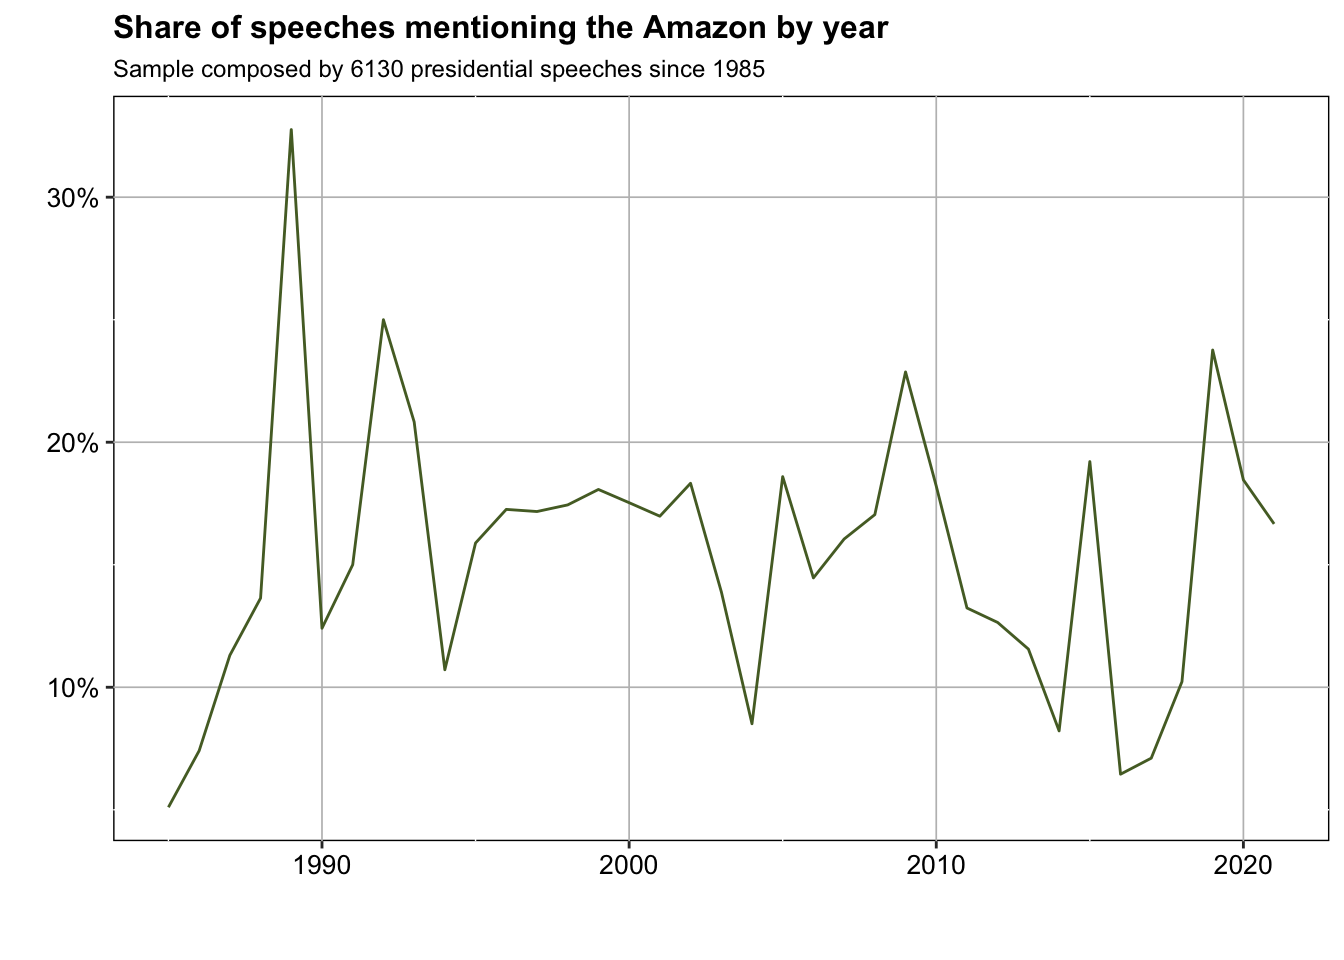
\includegraphics{Full_draft_20220401_files/figure-latex/Amazonian speeches by year-1.pdf}

While in 1990 there was a decrease to about 12.4\%, we observe a novel
increase to 15\% and 25\% in 1991 and 1992 respectively. The driver of
this increase is likely to be the 1992 Earth Summit, which was being
prepared by various state and non-state actors in the region and brought
international attention to environmental topics in Brazil. One of the
big announcements was the consolidation of the first transnational
partnership for the Amazon, the G7 Pilot Programme, which brought a high
number of financial resources to the region for public policy
implementation (cite). During the Cardoso years (1994-2002), Amazonian
speeches averaged at about 15\% without strong variation. There were no
big international or domestic events that drove the topic up.

We observe an increase from 8.5\% in 2004 to 22.8\% in the year of the
Copenhagen Summit, 2009. This coincides with the Presidency of Lula and
the steepest decrease in deforestation rates in Brazilian history. Lula
led the delegation to Copenhagen with a self-image of ``we do not
promise, we deliver'' (Franchini and Viola 2019), when stakes about
climate change were high. A somewhat different pattern can be identified
in the lead up to the 2015 Paris COP, which was also building up to
become a key-turn in climate politics after the failures of Copenhagen.
From 2010 to 2014, we identify a steady decrease from 18.2\% to 8.2\%,
which is followed by a sharp increase in the year of the COP, reaching
19.2\%. These are the years when Brazil entered a long period of
political and economic instability that lingers until today. Brazil went
to the COP in Paris with deforestation numbers slightly higher than
Copenhagen, and a perception that there was a turn towards less
conservation after the 2011 Forest Code was adopted.

We subsequently observe a steady increase from 6.4\% in 2016 to almost
24\% in the first year of Bolsonaro's presidency, 2019. As the narrative
of the climate crisis picks up in the late 2010s, international media
attention about the Amazon blasts, reaching unprecedented coverage.
Pictures of the Amazon on fire and of the red sky afternoon in São Paulo
circulated in social media and international media outlets in 2019.
President Bolsonaro engages in an international debacle with President
Macron and others, which drove the topic up strongly in the presidential
agenda. President Bolsonaro retrieves Brazil's hosting status for COP25,
and a strong process of dismantling of environmental governance starts
taking place.

We do find evidence that deforestation rates, economic situation,
elections, and simply preferential preferences affect the incidence of
Amazon in speeches: the smoothed curve portrays lower proportions
overall. However, international events and media coverage also correlate
with local maxima of our curve, suggesting presidents do speak more
about the Amazon in preparation or reaction to these events. We are yet
to inspect, though, whether specific problem constructions about the
Amazon change over time.

\hypertarget{amazonian-problem-construction-in-time}{%
\subsection{4.2 Amazonian problem-construction in
time}\label{amazonian-problem-construction-in-time}}

Figure 2 portrays plots with the proportions of different problem
constructions over time. We conceptualize four problem constructions:
sovereignty, economic integration, social development, and conservation.
At the level of the Amazonian statement, though, presidents might mix
two or more together. These are what we call mixed types, in opposition
to pure types. There are 16 mix types in total, and figure 2 portrays
the most frequent of them. Pure problem constructions dominate, with
their joint average above 55\%. Among the four pure types as well as the
mixed types, we observe a strong variation over time, suggesting the
narratives do respond differently to factors that affect Amazonian
statements discussed in the section above.

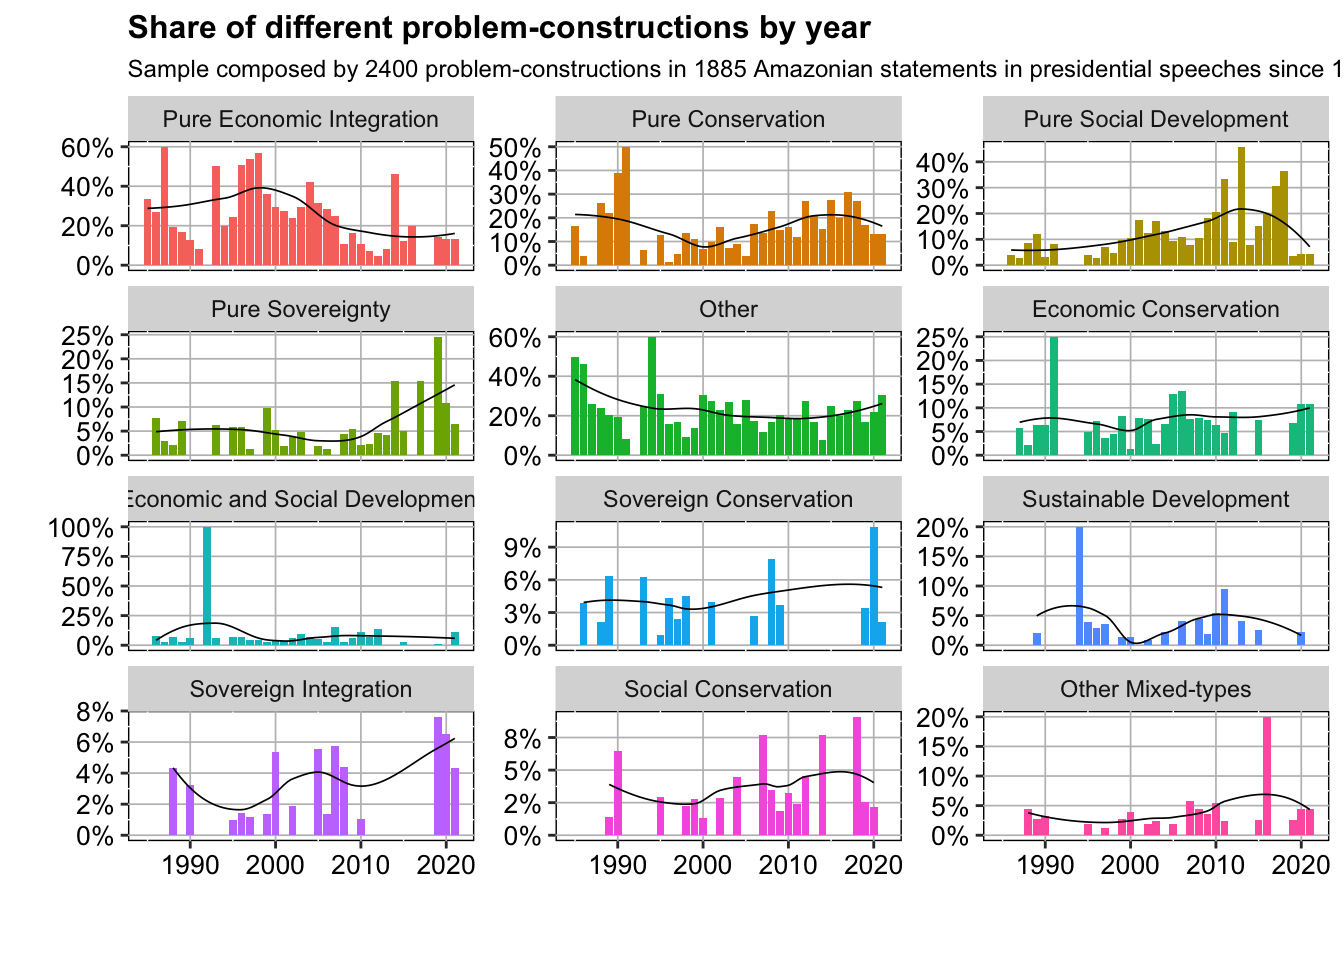
\includegraphics{Full_draft_20220401_files/figure-latex/mixed-types in time-1.pdf}

The plots reveal several trends. Pure economic integration statements,
which were dominant, decreased in incidence as of the mid 1990s. In the
late 1990s, pure conservation as well as pure social development
increased; both surpassing the proportion of economic integration
problem-construction in 2005. Capobianco (2021) argues that the
unprecedented decrease in deforestation we observed from 2004 to 2012
was a product of an increase in the perception of stronger federal
policies and presence in the Amazon region, which in turn engendered a
perception of higher risk of being caught and fined for deforestation.
This is aligned with our findings: a higher incidence of the Amazon as a
topic overall can generate a perception of more attention from the top,
and a shift from economic integration to conservation can generate a
perception of higher change of being caught. As of the early 2010s, we
observe a reversal of the trend with a twist: economic integration
starts picking up again in detriment of conservation and social
development problem constructions, but with sovereignty increasing
steadily.

Figure 3 (below) shows these shifts more clearly and highlights the
decrease of economic integration and increase of social and conservation
problem constructions preceding Lula's presidential mandate. Relatedly,
figure 3 also shows that while the reversal precedes the mandate of
President Bolsonaro, it was with him and his dismantling of social and
environmental policies that sovereignty and economic integration appears
the most, in detriment of social development and environmental
conservation. The starkest decrease relates to social development
construction between Temer's and Bolsonaro's administration.

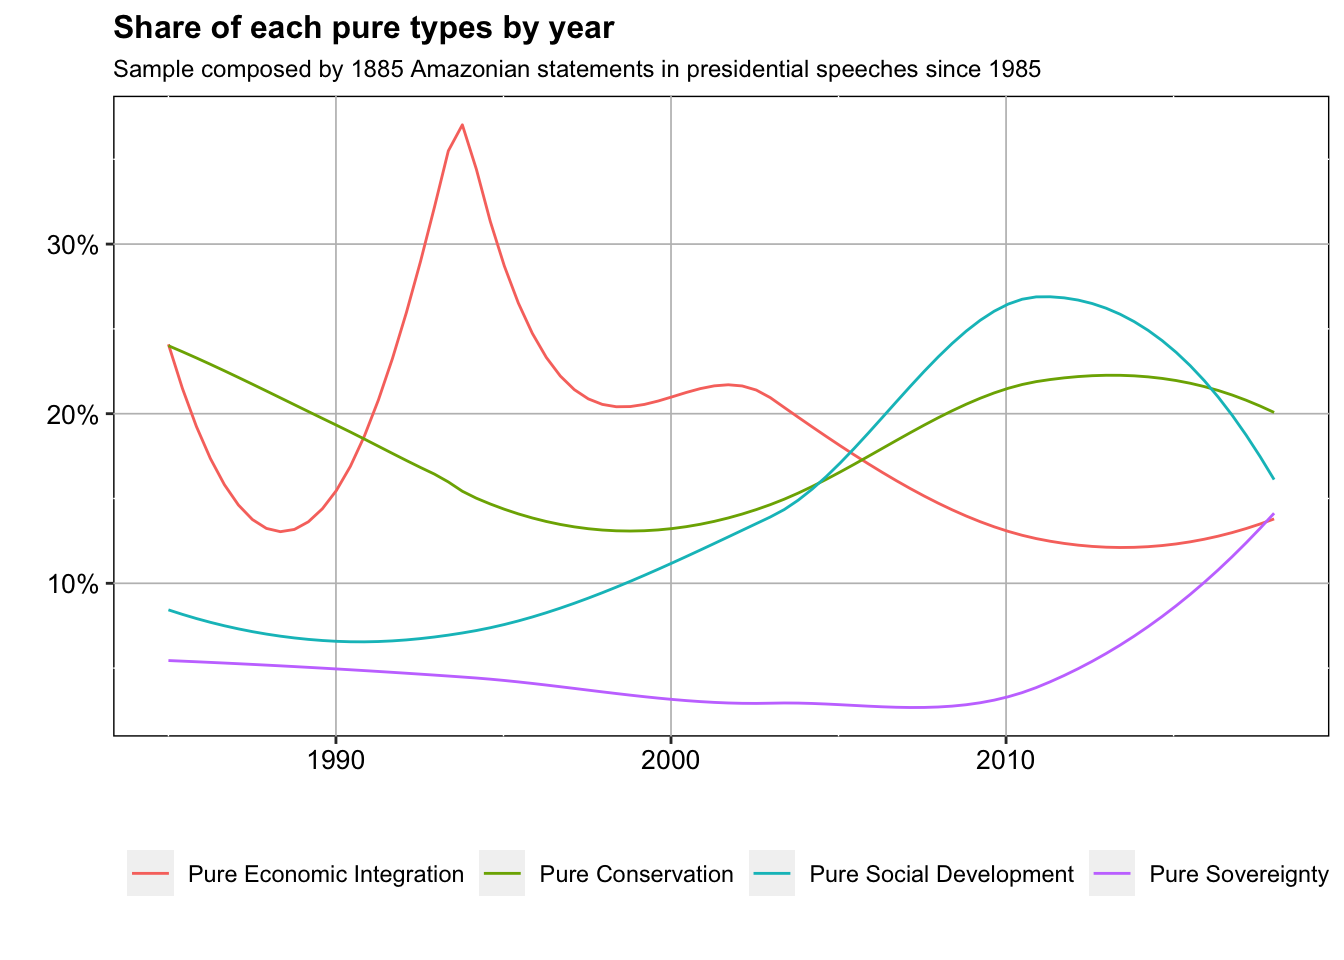
\includegraphics{Full_draft_20220401_files/figure-latex/pure types in time -1.pdf}

We now move to mixed types, which average at around 17\% for all
presidents in our sample: overall, presidents prefer pure
problem-constructions. While there is some variation in time for each
single mixed type, some of them have low counts and interpretations are
not adequate. We focus our discussion on those with higher incidence.
First, the most frequent mix overall is that of economic integration
with conservation, which after reaching 25\% of all
problem-constructions in 1989, remained stable at 9\% on average for the
remainder of the period. President Lula was the most frequent user of
this mix. Second, except for economic and social development appearing
together in all statements made by Color in 1992, mixed types using
conservation were quite frequent in the lead up and aftermath of the
1992 Earth Summit. This includes the mix type we label sustainable
development, which constructs the Amazon as a problem of economic
integration, social development, and environmental conservation. In all,
we interpret the appearance of mixed types as more complex
understandings of Amazonian problems. This follows a global agenda of
understanding interconnections of social, environmental, and economic
domains. As we show that Amazonian incidence in discourse does respond
to global issues, this is not a surprise given agendas as Millennium
Development Goals and the Sustainable Development Goals. Nevertheless,
as in pure types, we also observe the comeback of sovereignty being used
in mixed types in detriment of conservation. This becomes more apparent
in a comparison between Lula and Bolsonaro, the two presidents that mix
the most with proportions 11\% above presidential averages: 28.5\% and
28.6\% respectively. While the former frequently mixed conservation with
other problem constructions, the latter prefers mixing sovereignty. The
combination of sovereignty with economic integration, which was also
characteristic of the military dictatorship policies for the region,
reaches its highest level with Bolsonaro.

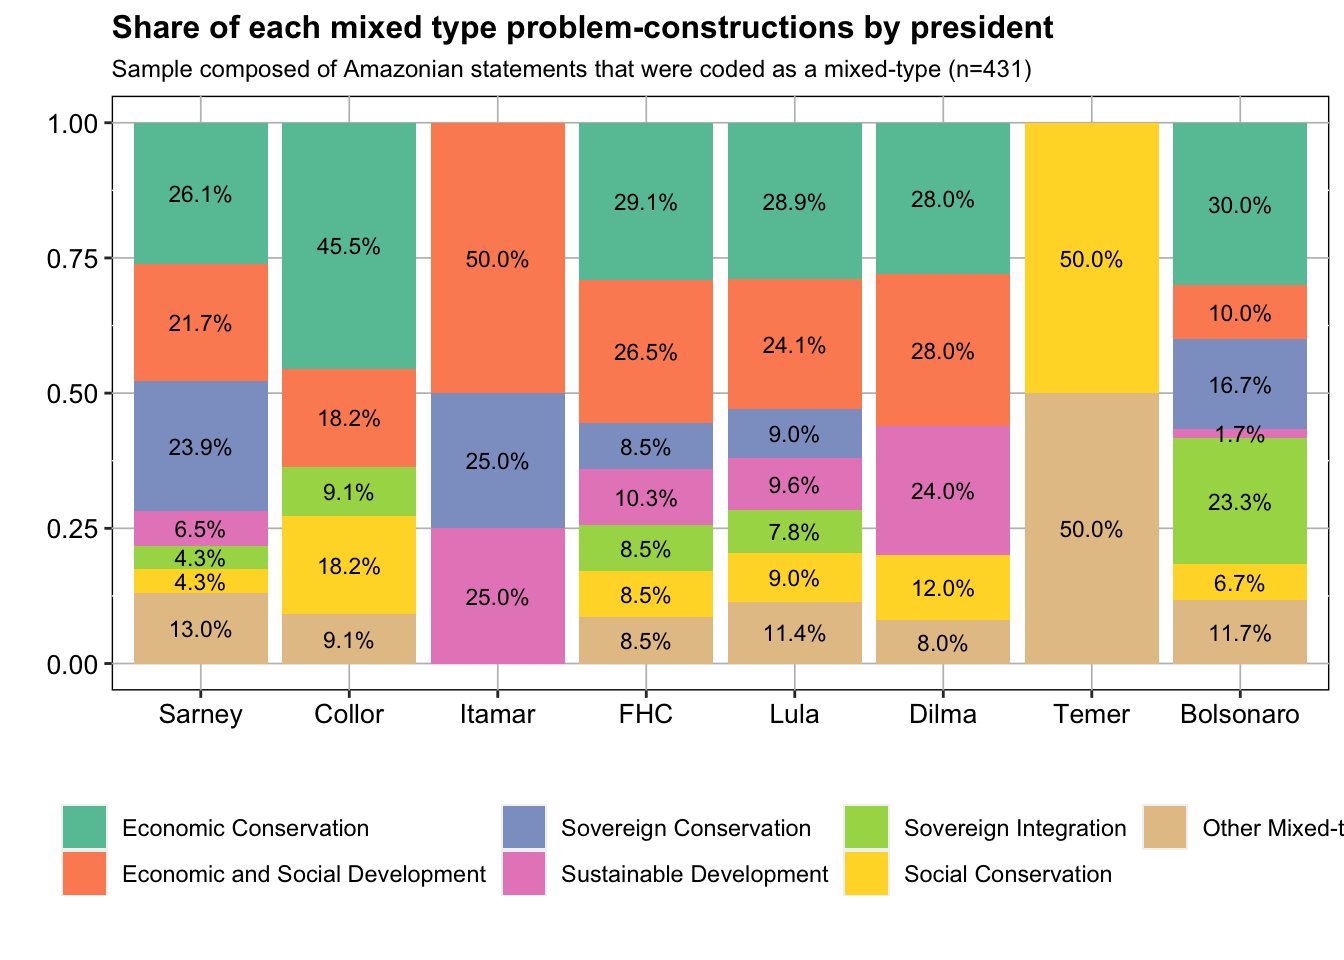
\includegraphics{Full_draft_20220401_files/figure-latex/mixed-types by president -1.pdf}

Pacheco (2019) proposes that we see the Amazon frontier as a key
analytic category to understand the Brazilian state and democracy.
Specifically, the author states that the natural richness of the region
has been instrumentally transformed in political support through
resource exploration by different governments over the last centuries.
The costs for said economic and political benefits are the livelihoods
of indigenous and traditional populations and the ecosystems they reside
in. Political stability, thus, can be seen as a product of the trade-off
between both. Policies during the military dictatorship were strongly
geared towards integrating the Amazon to the national territory and
international economy. With the strengthening of environmentalism in the
1990s, its most strong form being the policies adopted in the 2000s, we
can interpret the fall of economic integration and the rise of social
and conservation problem constructions as a new relationship between
granting local livelihoods their rights and economic exploitation.

While unprecedented, this new balance was not long-standing. Democratic
decay is slow and the embryony of Bolsonaro's Amazonian discourse was
breeding half a decade before he took office. We observe the decrease in
conservation related statements in the early 2010s, and the soft
increase of sovereignty in form of mixes in the mid 2000s. The hard
increase in sovereignty comes in the 2010s. As we conceptualize and
operationalize sovereignty as boundary-making vis-à-vis internal and
external perceived threats to the Amazon, we interpret this increase as
attacks to indigenous and traditional populations. At the policy side,
the Itaipu Dam in the late 2000s and the 2011 Forest code are seen as a
turning point: political opposition to conservation got particularly
organized and managed to lobby the executive and conquer this policy
wins, which were largely opposed by environmentalists.

This is not to say that those who preceded President Bolsonaro are like
him. They are not, and we have shown how he is different from others
already. But the political forces in Brazilian democracy that drive
these changes in problem-construction were long in the making, as the
earlier and softer shifts in discourse suggest. Bolsonaro's
problem-construction is the strongest form of this shift. Now that we've
inspected and developed pure and mixed types, we can check if these
specific problem constructions vary depending on where the president is
speaking.

\hypertarget{an-amazonian-three-level-game-boasting-policy-outside-talking-to-people-inside}{%
\subsection{4.3 An Amazonian three-level game? Boasting policy outside,
talking to people
inside}\label{an-amazonian-three-level-game-boasting-policy-outside-talking-to-people-inside}}

\hypertarget{conclusion}{%
\section{5 Conclusion}\label{conclusion}}

\hypertarget{references}{%
\section*{6 References}\label{references}}
\addcontentsline{toc}{section}{6 References}

\hypertarget{refs}{}
\begin{CSLReferences}{1}{0}
\leavevmode\vadjust pre{\hypertarget{ref-acker2014}{}}%
Acker, Antoine. 2014. {``{"}O maior incêndio do planeta{"}: como a
Volkswagen e o regime militar brasileiro acidentalmente ajudaram a
transformar a Amazônia em uma arena política global.''} \emph{Revista
Brasileira de História} 34 (December): 13--33.
\url{https://doi.org/10.1590/S0102-01882014000200002}.

\leavevmode\vadjust pre{\hypertarget{ref-acker2021}{}}%
---------. 2021. {``Amazon Development,''} Oxford research encyclopedia
of latin american history.,.
\url{https://doi.org/10.1093/acrefore/9780199366439.013.837}.

\leavevmode\vadjust pre{\hypertarget{ref-alesina2009}{}}%
Alesina, Alberto F., and Paola Giuliano. 2009. {``Preferences for
Redistribution.''} \url{https://www.nber.org/papers/w14825}.

\leavevmode\vadjust pre{\hypertarget{ref-andonova2014}{}}%
Andonova, Liliana B. 2014. {``Boomerangs to Partnerships? Explaining
State Participation in Transnational Partnerships for Sustainability.''}
\emph{Comparative Political Studies} 47 (3): 481--515.
\url{https://doi.org/10.1177/0010414013509579}.

\leavevmode\vadjust pre{\hypertarget{ref-assunuxe7uxe3o2015}{}}%
Assunção, Juliano, Clarissa Gandour, and Rudi Rocha. 2015.
{``Deforestation Slowdown in the Brazilian Amazon: Prices or
Policies?''} \emph{Environment and Development Economics} 20 (6):
697--722. \url{https://doi.org/10.1017/S1355770X15000078}.

\leavevmode\vadjust pre{\hypertarget{ref-bacchi2009}{}}%
Bacchi, Carol Lee. 2009. \emph{Analysing Policy: What's the Problem
Represented to Be?} Pearson.

\leavevmode\vadjust pre{\hypertarget{ref-barros2020}{}}%
Barros, Antonio Teixeira de. 2020. {``Discursos parlamentares sobre a
Amazônia: sobre o que falam os deputados brasileiros.''} \emph{Política
\& Sociedade} 19 (46): 299--331.
\url{https://doi.org/10.5007/2175-7984.2020.e66962}.

\leavevmode\vadjust pre{\hypertarget{ref-becker2005}{}}%
Becker, Bertha K. 2005. {``Geopolítica da Amazônia.''} \emph{Estudos
Avançados} 19 (April): 71--86.
\url{https://doi.org/10.1590/S0103-40142005000100005}.

\leavevmode\vadjust pre{\hypertarget{ref-bevitori2015}{}}%
Bevitori, Cinzia. 2015. {``Discursive Constructions of the Environment
in American Presidential Speeches 1960{\textendash}2013: A Diachronic
Corpus-Assisted Study.''} \emph{Corpora and Discourse Studies}, 110--33.
\url{https://doi.org/10.1057/9781137431738_6}.

\leavevmode\vadjust pre{\hypertarget{ref-brice2021}{}}%
Brice, and Smith. 2021. {``The Amazon Is Fast Approaching a Point of No
Return.''} \emph{Bloomberg.com}, July.
\url{https://www.bloomberg.com/news/features/2021-07-29/amazon-rainforest-deforestation-land-grabs-surge-under-bolsonaro-in-brazil}.

\leavevmode\vadjust pre{\hypertarget{ref-brown2017}{}}%
Brown, George, and Benjamin K. Sovacool. 2017. {``The Presidential
Politics of Climate Discourse: Energy Frames, Policy, and Political
Tactics from the 2016 Primaries in the United States.''} \emph{Energy
Policy} 111 (December): 127--36.
\url{https://doi.org/10.1016/j.enpol.2017.09.019}.

\leavevmode\vadjust pre{\hypertarget{ref-calderwood2019}{}}%
Calderwood, Kevin J. 2019. {``Discourse in the Balance: American
Presidential Discourse about Climate Change.''} \emph{Communication
Studies} 70 (2): 235--52.
\url{https://doi.org/10.1080/10510974.2019.1572636}.

\leavevmode\vadjust pre{\hypertarget{ref-calderwood2020}{}}%
---------. 2020. {``Going Global: Climate Change Discourse in
Presidential Communications.''} \emph{Environmental Communication} 14
(1): 52--67. \url{https://doi.org/10.1080/17524032.2019.1592005}.

\leavevmode\vadjust pre{\hypertarget{ref-campbell2015}{}}%
Campbell, Jeremy M. 2015. \emph{Conjuring Property: Speculation and
Environmental Futures in the Brazilian Amazon}. Illustrated edition.
Seattle: University of Washington Press.

\leavevmode\vadjust pre{\hypertarget{ref-capobianco2019}{}}%
Capobianco, João Paulo. 2019. {``Avances y retrocesos de la
sostenibilidad en la Amazonia: un análisis de la gobernanza
socioambiental en la Amazonia,''} January.
\url{https://gredos.usal.es/handle/10366/139311}.

\leavevmode\vadjust pre{\hypertarget{ref-capobianco2021}{}}%
---------. 2021. \emph{Amazônia: Uma Década de Esperança}. 1ª edição.
São Paulo: Estação Liberdade.

\leavevmode\vadjust pre{\hypertarget{ref-drummond2006}{}}%
Drummond, Jose, and Ana Flavia Barros-Platiau. 2006. {``Brazilian
Environmental Laws and Policies, 1934-2002: A Critical Overview.''}
\emph{Law \textless Html{\_}ent Glyph={"}@amp;{"}
Ascii={"}\&amp;{"}/\textgreater{} Policy} 28 (1): 83--108.
\url{https://doi.org/10.1111/j.1467-9930.2005.00218.x}.

\leavevmode\vadjust pre{\hypertarget{ref-franchini2019}{}}%
Franchini, Matias Alejandro, and Eduardo Viola. 2019. {``Myths and
Images in Global Climate Governance, Conceptualization and the Case of
Brazil (1989 - 2019).''} \emph{Revista Brasileira de Política
Internacional} 62 (September).
\url{https://doi.org/10.1590/0034-7329201900205}.

\leavevmode\vadjust pre{\hypertarget{ref-garfield2013}{}}%
Garfield, Seth. 2013. \emph{In Search of the Amazon: Brazil, the United
States, and the Nature of a Region}. Durham: Duke University Press
Books.

\leavevmode\vadjust pre{\hypertarget{ref-harris2021}{}}%
Harris, Bryan. 2021. {``Drought Puts Amazon at Risk of {`}Large-Scale
Dieback{'}, Researchers Warn.''} \emph{Financial Times}, July.
\url{https://www.ft.com/content/02071ae7-dcf5-4c61-9c3c-b55f5aef8b0e}.

\leavevmode\vadjust pre{\hypertarget{ref-hecht2013}{}}%
Hecht, Susanna B. 2013. \emph{The Scramble for the Amazon and the
{"}Lost Paradise{"} of Euclides Da Cunha}. First edition. Chicago:
University of Chicago Press.

\leavevmode\vadjust pre{\hypertarget{ref-hecht1990}{}}%
Hecht, Susanna B., and Alexander Cockburn. 1990. \emph{The Fate of the
Forest: Developers, Destroyers, and Defenders of the Amazon, Updated
Edition}. Chicago, IL: University of Chicago Press.
\url{https://press.uchicago.edu/ucp/books/book/chicago/F/bo10387801.html}.

\leavevmode\vadjust pre{\hypertarget{ref-hirschman1963}{}}%
Hirschman, Albert O. 1963. \emph{Journeys Toward Progress: Studies of
Economic Policy-Making in Latin America}. Twentieth Century Fund.

\leavevmode\vadjust pre{\hypertarget{ref-hirschman1975}{}}%
---------. 1975. {``Policymaking and Policy Analysis in Latin America: A
Return Journey.''} \emph{Policy Sciences} 6 (4): 385--402.
\url{https://www.jstor.org/stable/4531616}.

\leavevmode\vadjust pre{\hypertarget{ref-hochstetler2021}{}}%
Hochstetler, Kathryn. 2021. {``Climate Institutions in Brazil: Three
Decades of Building and Dismantling Climate Capacity.''}
\emph{Environmental Politics} 30 (sup1): 49--70.
\url{https://doi.org/10.1080/09644016.2021.1957614}.

\leavevmode\vadjust pre{\hypertarget{ref-hochstetler2007}{}}%
Hochstetler, Kathryn, and Margaret E. Keck. 2007. \emph{Greening Brazil:
Environmental Activism in State and Society}.
\url{https://doi.org/10.1215/9780822390596}.

\leavevmode\vadjust pre{\hypertarget{ref-miranda2021}{}}%
Miranda, David. 2021. {``Bolsonaro{'}s 1,000km Amazon Railway Will Cause
Climate Chaos. It Must Be Stopped.''} \emph{The Guardian}, July.
\url{https://www.theguardian.com/commentisfree/2021/jul/28/bolsonaro-amazon-railway-climate-chaos-must-be-stopped}.

\leavevmode\vadjust pre{\hypertarget{ref-pacheco2019}{}}%
Pacheco, João. 2019. \emph{Ecxterminio y Tutela: Procesos de Formación
de Alteridades En El Brasil}. UNSAM Edita. Ciencias sociales.
\url{http://www.unsamedita.unsam.edu.ar/product/exterminio-y-tutela-procesos-de-formacion-de-alteridades-en-el-brasil/}.

\leavevmode\vadjust pre{\hypertarget{ref-lepolaindewaroux2021}{}}%
Polain de Waroux, Yann le, Rachael D. Garrett, Mollie Chapman, Cecilie
Friis, Jeffrey Hoelle, Leonie Hodel, Kelly Hopping, and Julie Gwendolin
Zaehringer. 2021. {``The Role of Culture in Land System Science.''}
\emph{Journal of Land Use Science} 16 (4): 450--66.
\url{https://doi.org/10.1080/1747423X.2021.1950229}.

\leavevmode\vadjust pre{\hypertarget{ref-putnam1988}{}}%
Putnam, Robert D. 1988. {``Diplomacy and Domestic Politics: The Logic of
Two-Level Games.''} \emph{International Organization} 42 (3): 427--60.
\url{https://www.jstor.org/stable/2706785}.

\leavevmode\vadjust pre{\hypertarget{ref-silva-muller2022}{}}%
Silva-Muller, Livio, and Moira Faul. 2022. {``Protecting the Amazon and
Its People: The Role of Civil Society in the Local Effectiveness of
Transnational Partnerships.''} In, 1st ed., 288. Routledge Research in
Environmental Policy and Politics. Taylor; Francis Routledge.
\url{https://www.routledge.com/Partnerships-for-Sustainability-in-Contemporary-Global-Governance-Pathways/Andonova-Faul-Piselli/p/book/9780367708870\#:~:text=\%22Partnerships\%20for\%20Sustainability\%20provides\%20a,collaboration\%20of\%20public\%20and\%20private.}

\leavevmode\vadjust pre{\hypertarget{ref-westerwinter2021}{}}%
Westerwinter, Oliver. 2021. {``Transnational Public-Private Governance
Initiatives in World Politics: Introducing a New Dataset.''} \emph{The
Review of International Organizations} 16 (1): 137--74.
\url{https://doi.org/10.1007/s11558-019-09366-w}.

\leavevmode\vadjust pre{\hypertarget{ref-zarefsky2004}{}}%
Zarefsky, David. 2004. {``Presidential Rhetoric and the Power of
Definition.''} \emph{Presidential Studies Quarterly} 34 (3): 607--19.
\url{https://www.jstor.org/stable/27552615}.

\end{CSLReferences}

\end{document}
